\documentclass[a4paper,reqno,12pt]{report}
\usepackage{amsmath, amsthm, amssymb, graphicx, caption, booktabs}
\usepackage[bottom]{footmisc}
\usepackage{url}
\usepackage[section]{placeins}
\usepackage{float}
\usepackage{listings}
\usepackage{color}
\usepackage{nameref}
\usepackage{gensymb}
\usepackage[nottoc]{tocbibind}
\usepackage{titlesec}
\usepackage{csquotes}
\usepackage{wrapfig}
\usepackage{appendix}
\usepackage{subcaption}
\usepackage{algorithm}
\usepackage{tabularx}
\usepackage{graphicx}
\usepackage{adjustbox}
\usepackage[noend]{algpseudocode}

\definecolor{mygreen}{rgb}{0,0.6,0}
\definecolor{mygray}{rgb}{0.5,0.5,0.5}
\definecolor{mymauve}{rgb}{0.58,0,0.82}

\lstset{ %
  backgroundcolor=\color{white},   % choose the background color
  basicstyle=\footnotesize,        % size of fonts used for the code
  breaklines=true,                 % automatic line breaking only at whitespace
  captionpos=b,                    % sets the caption-position to bottom
  commentstyle=\color{mygreen},    % comment style
  escapeinside={\%*}{*)},          % if you want to add LaTeX within your code
  keywordstyle=\color{blue},       % keyword style
  stringstyle=\color{mymauve},     % string literal style
}

\begin{document}

\title{%
  MATH3531\\
  Simulation and Modelling\\
  Final Project\\
  Monopoly
  }
\author{(Wallace) Mackenzie Chase\\
Andrew MacKenzie}
\date{\today}
\maketitle
\clearpage

\section*{\underline{Introduction}}
For our final project, we decided to do monopoly.
\\
Our design is relatively simple. We utilized Player, Tile, and Game classes and a main loop to simulate games of Monopoly.
Games will run until a player has won, or the last player to still have money. We have a HouseRules option to toggle if games use the house rules or not.\\
One issue we ran into was games running forever as the initial rents are too low. Players are able to make their way around the board and pass GO, collecting \$200 faster than they can lose the money in rent. To resolve this, we just created an inflation variable that increases the rent every 50 turns. This decision was arbitrary and can be changed to observe changes in the results.
\\
Our base scenario or control, is 50,000 games with 4 players, and an inflation rate of +1 in rent every 50 turns.
\\
We then ran the program changing the amount of games, the amount of players, and the inflation rate and observed the changes.
\section*{\underline{Results}}
\begin{table}[htbp]
\begin{adjustbox}{width=\textwidth}
\begin{tabular}{ |c|c|c|c|c|c|c|c| }
\hline
Scenario & Games & Players & Inflation & House Rules & Average Turns & Order Matters & average trip\\
\hline
Control & 50,000 & 4 & 50 turns +1 & OFF & 485 & YES & 20\\ 
Control & 50,000 & 4 & 50 turns +1 & ON & 552 & YES & 30\\
\hline
More Games & 100,000 & 4 & 50 turns +1 & OFF & 485 & YES & 20\\ 
More Games & 100,000 & 4 & 50 turns +1 & ON & 553 & YES & 30\\ 
\hline
Less Players & 50,000 & 2 & 50 turns +1 & OFF & 139 & NO & 1\\ 
Less Players & 50,000 & 2 & 50 turns +1 & ON & 553 & YES & 13\\ 
\hline
Higher Inflation & 50,000 & 4 & 50 turns +3 & OFF & 135 & YES & 6\\ 
Higher Inflation & 50,000 & 4 & 50 turns +3 & ON & 171 & YES & 6\\ 
\hline
\end{tabular}
\end{adjustbox}
\end{table}
From our findings, we see there is no difference in the amount of games played, the average turn per game remains the same, the order matters, Player 1 and 2 perform much better than players 3 and 4. The average amount of trips around the board before all properties are bought also remains the same.
\\
When we change the amount of players in the game, we notice a big difference when house rules are applied or not. When house rules are not used, the average amount of turns was 139, player order did not matter, and the average amount of trips before all properties were bought was 1. This is mostly due to a lot of games ending before all properties were bought. However, when the house rules were used, the order did matter, the average amount of turns went up as did the average trip before all properties were bought.
\\
Changing the inflation rate really only affected the average amount of turns for games and trips around the board before all properties were bought.
\\
\\
From this, we can conclude player order does matter, except for fewer players and no house rules. We can also say that the house rules do affect the average turns and average trip, however this would make sense as gaining \$500 dollars on free parking and not auctioning properties would extend the length of games and the amount of trips before all properties are bought.
\section*{\underline{Control}}
\begin{figure}[h]
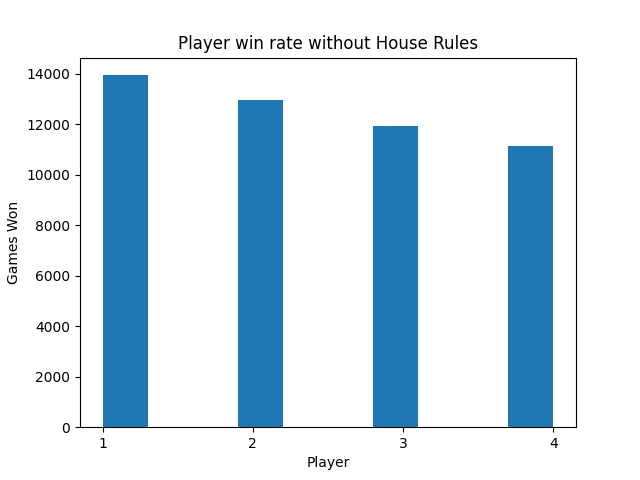
\includegraphics[width=15cm]{houseRulesOFF_50turns_+1_50000games.png}
\centering
\end{figure}
\begin{figure}[h]
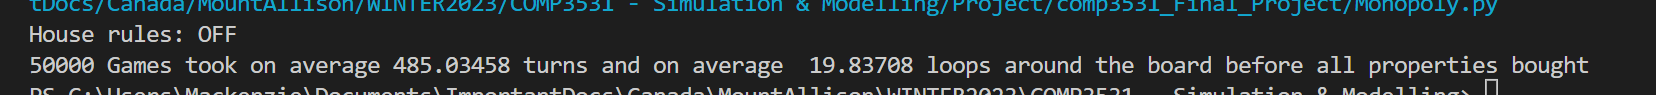
\includegraphics[width=15cm]{50000games_HouseRulesOFF_averages.png}
\centering
\end{figure}
\begin{figure}[h]
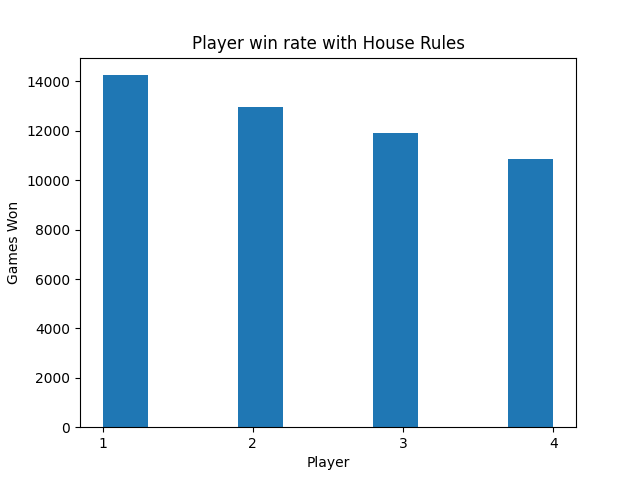
\includegraphics[width=15cm]{houseRulesON_50turns_+1_50000games.png}
\centering
\end{figure}
\begin{figure}[h]
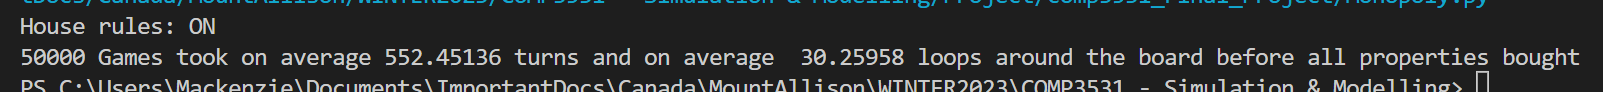
\includegraphics[width=15cm]{50000games_HouseRulesON_averages.png}
\centering
\end{figure}
\clearpage

\section*{\underline{More Games}}
\begin{figure}[h]
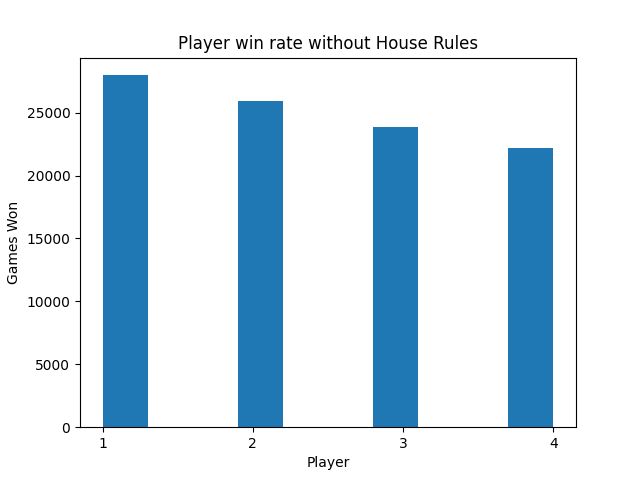
\includegraphics[width=15cm]{houseRulesOFF_50turns_+1_100000games.png}
\centering
\end{figure}
\begin{figure}[h]
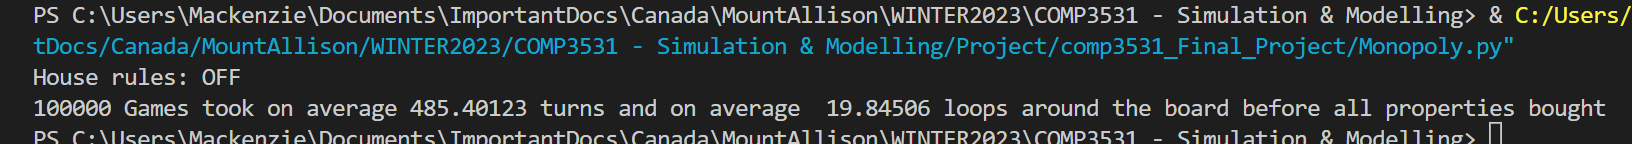
\includegraphics[width=15cm]{100000games_HouseRulesOFF_averages.png}
\centering
\end{figure}
\begin{figure}[h]
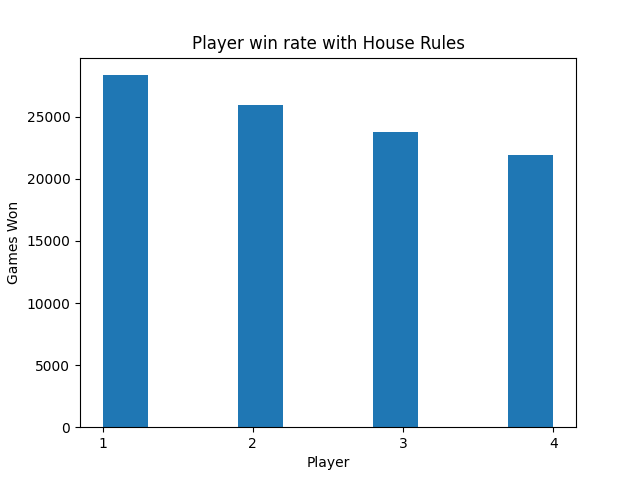
\includegraphics[width=15cm]{houseRulesON_50turns_+1_100000games.png}
\centering
\end{figure}
\begin{figure}[h]
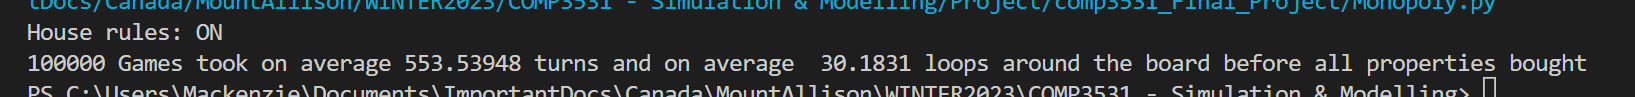
\includegraphics[width=15cm]{100000games_HouseRulesON_averages.png}
\centering
\end{figure}
\clearpage

\section*{\underline{Less Players}}
\begin{figure}[h]
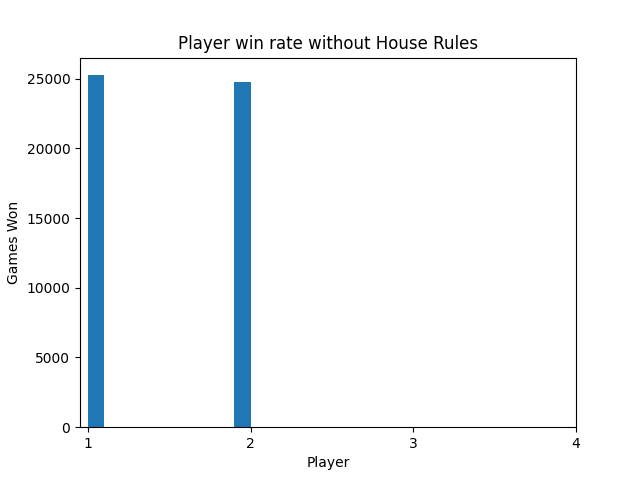
\includegraphics[width=15cm]{2_player_test_noHouseRules.png}
\centering
\end{figure}
\begin{figure}[h]
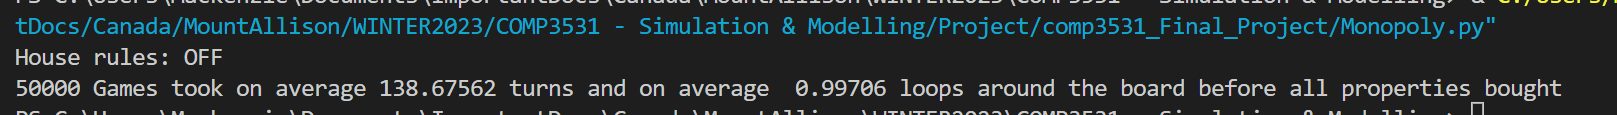
\includegraphics[width=15cm]{2_player_test_noHouseRules_averages.png}
\centering
\end{figure}
\begin{figure}[h]
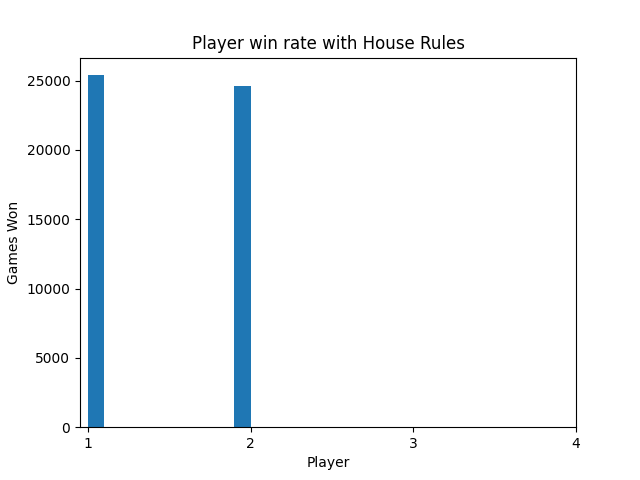
\includegraphics[width=15cm]{2_player_test.png}
\centering
\end{figure}
\begin{figure}[h]
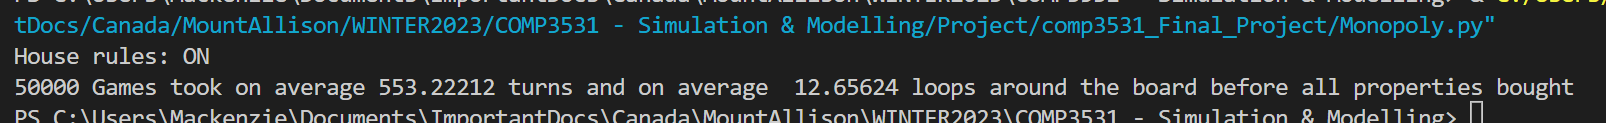
\includegraphics[width=15cm]{2_player_test_HouseRules.png}
\centering
\end{figure}
\clearpage

\section*{\underline{higher Inflation}}
\begin{figure}[h]
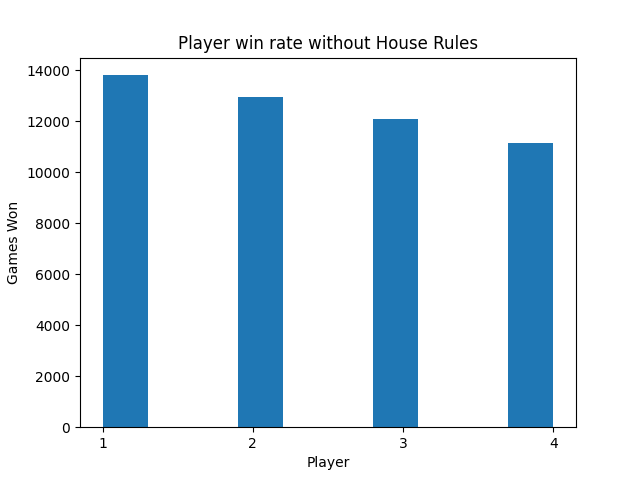
\includegraphics[width=15cm]{highInflation.png}
\centering
\end{figure}
\begin{figure}[h]
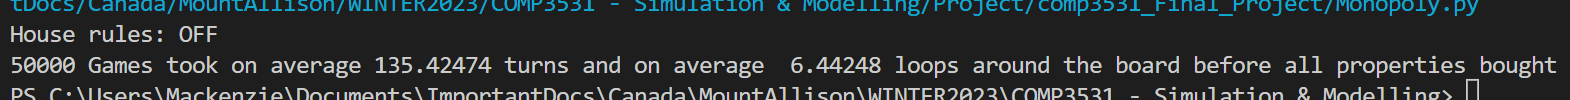
\includegraphics[width=15cm]{highInflation_averages.png}
\centering
\end{figure}
\begin{figure}[h]
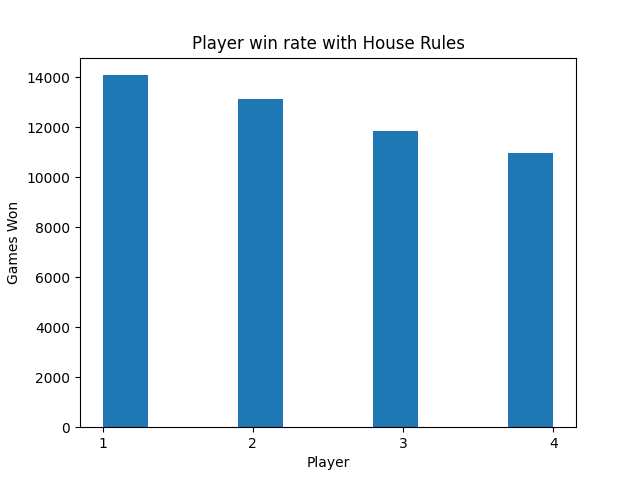
\includegraphics[width=15cm]{highInflation_houseRules.png}
\centering
\end{figure}
\begin{figure}[h]
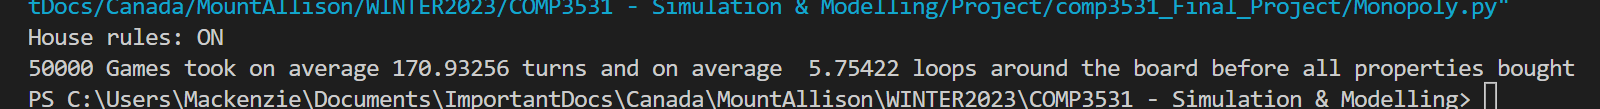
\includegraphics[width=15cm]{highInflation_houserules_averages.png}
\centering
\end{figure}
\clearpage
\end{document}
